\documentclass[tikz]{standalone}
\usepackage{mathtools}
\usetikzlibrary{angles, quotes, decorations.pathreplacing}

\begin{document}
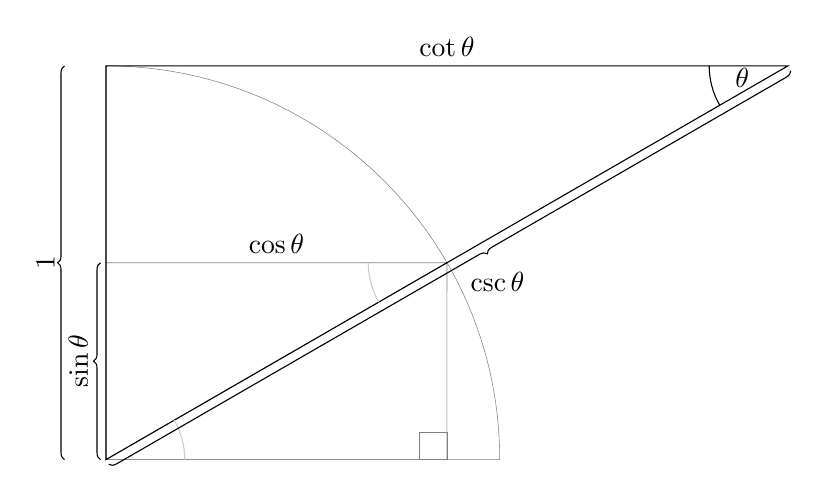
\begin{tikzpicture}[scale=5]
  \coordinate (A) at (0, 0);
  \coordinate (B) at (30:1);
  \coordinate (C) at (B |- {(1, 0)});

  \coordinate (Bp) at ({(0, 1)} |- B);
  \coordinate (Bpcsc) at (0, 1);
  \coordinate (Bcsc) at (30:{cosec(30)});

  \draw[help lines] (0, 1) -- (0, 0) --
    (1, 0) arc[start angle=0, end angle=90, radius=1] -- cycle;

  \draw[help lines] (A) -- (B) -- (C) -- cycle;

  \draw[help lines] (Bp) -- node[above, text=black] {$\cos\theta$} (B);

  \draw (A) -- (Bpcsc) -- node[above] {$\cot\theta$} (Bcsc) -- cycle;

  \draw pic[angle radius=10mm, draw=black!20!white] {angle=C--A--B};
  \draw pic[angle radius=10mm, draw=black!20!white] {angle=Bp--B--A};
  \draw pic[angle radius=10mm, draw=black, "$\theta$"] {angle=Bpcsc--Bcsc--A};
  \draw[help lines] (C) rectangle +(-2pt, 2pt);

  \draw[decorate, decoration={brace, raise=2pt}] (A) -- (Bp)
    node[midway, anchor=south, xshift=-3pt, rotate=90] {$\sin\theta$};
  \draw[decorate, decoration={brace, raise=15pt}] (A) -- (Bpcsc)
    node[midway, anchor=south, xshift=-15pt, rotate=90] {$1$};
  \draw[decorate, decoration={brace, raise=2pt, aspect=0.45}] (Bcsc) -- (A)
    node[midway, below right, xshift=5pt] {$\csc\theta$};
\end{tikzpicture}
\end{document}

%%% Local Variables:
%%% mode: latex
%%% TeX-master: t
%%% End:
